\documentclass[sanserif]{beamer}
%\documentclass[sanserif,handout]{beamer}
\usepackage [T1] {fontenc} 
\usepackage{pdfpages}
\usepackage{citesupernumber}
\usepackage{multirow}
\usepackage{pgfpages}
%\pgfpagesuselayout{4 on 1}[letterpaper, landscape, border, shrink=5mm]
\usepackage{graphicx}
\usepackage{tikz}
\usetikzlibrary{fit,positioning}

\hyphenpenalty=5000
\tolerance=1000


\definecolor{green}{rgb}{0.0,0.7,0.0}
\setbeamercolor{green}{fg=green}
\setbeamercolor{gray}{fg=gray} 
\setbeamercolor{red}{fg=red}
\setbeamercolor{black}{fg=black}
\setbeamercolor{white}{fg=white}
\definecolor{unf}{rgb}{0.0,0.2,0.9}
\definecolor{poz}{rgb}{0.7,0.7,0.0}
\definecolor{neg}{rgb}{0.7,0.0,0.0}
\setbeamercolor{unf}{fg=unf}
\setbeamercolor{poz}{fg=poz}
\setbeamercolor{neg}{fg=neg}


\setbeamerfont{italic}{shape=\slshape}
\setbeamerfont{upright}{shape=\upshape}
\setbeamerfont{tt}{family=\ttfamily}
\setbeamerfont{rm}{family=\sffamily}
\setbeamerfont{bold}{series=\bfseries}
\setbeamerfont{norm}{series=\normalfont}
\setbeamerfont{tiny}{size=\tiny}
\setbeamerfont{small}{size=\small}
\setbeamerfont{normal}{size=\normalsize}



\setbeamerfont{frametitle}{series=\bfseries}
\setbeamertemplate{bibliography item}[text]

\newcommand{\EQU}{\texttt{equals}}
\newcommand{\LogicNine}{\texttt{Logic-9}}
\newcommand{\EquOnly}{\texttt{equals only}}
\newcommand{\gray}[1]{ \usebeamercolor[fg]{gray}#1\usebeamercolor{normal text}}
\newcommand{\italics}[1]{\usebeamerfont{italic}#1\usebeamerfont{upright}}
\renewcommand{\tt}[1]{\usebeamerfont{tt}#1\usebeamerfont{rm}}
\newcommand{\bolds}[1]{\usebeamerfont{bold}#1\usebeamerfont{norm}}
\newcommand{\li}[1]{\begin{tabular}{p{0.01\textwidth} p{0.40\textwidth}}  $\bullet$ & \usebeamerfont{small} #1 \end{tabular}}

\setbeamertemplate{navigation symbols}{ \insertframenumber } 

\mode<presentation>
{
	\usetheme{Berkeley}
	\usecolortheme{orchid}
}

\title[Evolvability]{On the Evolution of\\Evolvability}
\author[]{Rosangela Canino-Koning}
\date{Wednesday 09 December 2015}

\begin{document}
\bibliographystyle{nature}

\frame{\titlepage}

%%%%%%%%%%%%%%%%%% INTRODUCTION %%%%%%%%%%%%%%%%%%%
\section[Introduction]{Introduction}

\frame{
	\frametitle{What is Evolvability?}
	\begin{block}{Evolvability}
	"The potential of populations and genomes to produce adaptive variation and complex structures in response to mutation and selection."
	\end{block}
	\note{obviously, this isn't an obvious definition. so much controversy}
}

\subsection[Historical Context]{Historical Context}

\frame{
   \frametitle{Heritability and Response to Selection}
   \begin{block}{Fisher and Wright
   		\cite{fisher_genetical_1930,wright_evolution_1931}
   		}

   	Narrow-sense Heritability
   	\begin{equation}
   	h^2 = \frac{Var_A}{Var_P}
   	\end{equation}
   	The Breeder's Equation
   \begin{equation}
   R = {h^2}S
   \end{equation}
	\end{block}
}

\frame{
	\frametitle{Modern Synthesis - Genetic Coefficient of Variation as a measure of Evolvability}
	
	\begin{quotation}
		"There are two distinct kinds of questions that require comparing standardized estimates of genetic variation: first how fast will a character respond to a given selective pressure; and second how much variability is maintained in relation to the evolutionary forces which act on it. In both these cases, evolvability and variability, I suggest that the genetic coefficient of variation $CV_a$, provides a great deal of relevant information."
		
		-- Houle (1992)\cite{houle_comparing_1992} 
	\end{quotation}
}

\frame{
	\frametitle{Evolvable Embryologies}
	
	\begin{quotation}
		"Certain kinds of embryology find it difficult to generate certain kinds of biomorphs; other kinds of embryology find it easy to do so. It is clear that we have here a powerful analogy for something important about real biology, a major principle of real life that is illustrated by artificial life."
		
		--Dawkins (1989)\cite{dawkins_13_2003}
	\end{quotation}
		
	\begin{quotation}
		"[Evolvability] is a property of embryological systems, i.e., certain types of developmental systems are better at evolving. For example, the invention of multicellularity, segmentation or the sequestration of the germ line appear, with hindsight, to have been key developmental events that have speeded up the evolution"
		
		--Alberch (1991)\cite{alberch_genes_1991}
	\end{quotation}
	
	\note{cite KG}	
}


\frame{
	\frametitle{Variation vs Variability}

		\begin{quotation}
			"The term \textbf{variation} refers to the actually present differences among the individuals in a population or a sample, or between the species in a clade. Variation can be directly observed as a property of a collection of items. In contrast, \textbf{variability} is a term that describes the potential or the propensity to vary."			
				
				--Wagner and Altenberg (1996)
				%\cite{wagner_perspective_1996}
			\end{quotation}
}

\subsection[Concepts and Scope]{Scope and Context}

\frame{\frametitle{Broad Concepts of Evolvability, varying in scale and effect}
		\usebeamerfont{small}
	\begin{tabular}{|c|c|c|}
		\hline \textbf{Suggested Term} & \textbf{Scale} & \textbf{Description and Effects} \\
		\hline \parbox[t]{2.5cm}{Heritability \\(\textit{sensu} Houle\cite{houle_comparing_1992})}  &  \parbox[t]{2cm}{Within\\ Populations}  & \parbox[t]{3.5cm}{Standing pool of genetic variation - determines response to selection} \\ 
		\hline \parbox[t]{2.5cm}{Evolvability \\(\textit{sensu} Wagner/Altenberg} & \parbox[t]{2cm}{Within\\Species} & \parbox[t]{3.5cm}{Variability, genetic architecture and developmental constraint - long-term adaptation, mid-term exploration of phenotypic space} \\ 
		\hline \parbox[t]{2.5cm}{Innovation \\(\textit{sensu} Maynard-Smith and Szathmary)\cite{smith_major_1995}} & \parbox[t]{2cm}{Within\\Clades} & \parbox[t]{3.5cm}{Potential to overcome genetic and developmental constraints - novelty generation } \\ 
		\hline 
	\end{tabular} 
	--Pigliucci (2008)\cite{pigliucci_is_2008}
}

\frame{\frametitle{Broad Concepts of Evolvability, varying in scale and effect}
	\usebeamerfont{small}
	\begin{tabular}{|c|c|c|}
		\hline \textbf{Suggested Term} & \textbf{Scale} & \textbf{Description and Effects} \\
		\hline \parbox[t]{2.5cm}{Heritability \\(\textit{sensu} Houle\cite{houle_comparing_1992})}  &  \parbox[t]{2cm}{Within\\ Populations}  & \parbox[t]{3.5cm}{Standing pool of genetic variation - determines response to selection} \\ 
		\hline \parbox[t]{2.5cm}{\usebeamercolor[fg]{red}Evolvability \\(\textit{sensu} Wagner/Altenberg} & \parbox[t]{2cm}{\usebeamercolor[fg]{red}Within\\Species} & \parbox[t]{3.5cm}{\usebeamercolor[fg]{red}Variability, genetic architecture and developmental constraint - long-term adaptation, mid-term exploration of phenotypic space} \\ 
		\hline \parbox[t]{2.5cm}{Innovation \\(\textit{sensu} Maynard-Smith and Szathmary)\cite{smith_major_1995}} & \parbox[t]{2cm}{Within\\Clades} & \parbox[t]{3.5cm}{Potential to overcome genetic and developmental constraints - novelty generation } \\ 
		\hline 
	\end{tabular} 
	--Pigliucci (2008)\cite{pigliucci_is_2008}
}

%%%%%%%%%%%%%%%%% SECTION %%%%%%%%%%%%%%%%%%%%%

\section[Definitions]{So, what is Evolvability}

\frame{
	\frametitle{So, what is Evolvability?}
	\begin{enumerate}
		\item Wagner/Alternberg Conception - Variability
		\item Organization of genetic components - Architecture
		\item Genotype/Phenotype Map
	\end{enumerate}
}

\frame{
	\frametitle{Modularity}
	\begin{block}{Levels of Modularity}
	\begin{enumerate}
		\item Spatial Modularity - less overlap of genetic sites for a pair of traits
		\item Functional Modularity - reduced pleiotropy between unrelated traits
		\item Trait Complexes - increased pleiotropic links within related sets of traits.
	\end{enumerate}
	\end{block}
}

\frame{
	\frametitle{Measuring Spatial Modularity}
\begin{quote}
	To measure Spatial Modularity, $m_S$:
	
	\begin{enumerate}
		\item count the total number of traits expressed in a genome: $T$
		\item identify the number of sites that code for any trait: set $K$
		\item count the number of items in set $K$: $k$
		\item count the number of traits coded for by each site within set $K$: $t_k$;
		\item calculate the inverse of the average number of traits coded for per site to reflect the level of spatial modularity ($m_S$) of coding regions of a genome
	\end{enumerate}
	\begin{equation}
	m_S = \frac{1}{\frac{1}{k} {\sum_{i=1}^{k} \frac{t_{k}}{T}}} 
	\end{equation}
\end{quote}
}

\frame{
	\frametitle{Robustness}
		\begin{block}{Types of Robustness}
			\begin{enumerate}
				\item Robustness to environmental perturbation
				\item Robustness to mutation
				\begin{enumerate}
					\item Genotypic Robustness
					\item Phenotypic Robustness
				\end{enumerate}
			\end{enumerate}
		\end{block}
}

\frame{
	\frametitle{Measuring Genotypic Robustness}
	
	\begin{quote}
		
		To measure Genotypic Robustness, $r_G$, of a genotype $G$:
		\begin{enumerate}
			\item count the number of loci in the genome: $n$
			\item count the number of possible alleles at a given site: $D$ 
			\item enumerate all possible single-step mutants that may arise from the given genotype (or sample from a more realistic distribution): $n(D-1)$;			
			\item count those mutants that prove to be neutral phenotypic variants: $R_G$;
			\item calculate the proportion of neutral phenotypic variants to reflect the probability of a neutral variant being produced by this genotype in response to mutation. 
			
		\end{enumerate}
		\begin{equation}
		r_{G} = \frac{R_{G}}{n(D-1)}
		\end{equation} 
	\end{quote}
	

}

\frame{
	\frametitle{Measuring Phenotypic Robustness}
\begin{quote}
	To measure Phenotypic robustness, $r_P$:
	
	\begin{enumerate}
		\item count the number of distinct neutral genetic variants that produce a given phenotypic trait in a population, ($Set K: k$);
		\item calculate the proportion of neutral variants produced by single-step mutations $r_G$, averaged over all of the neutral genetic variants to reflect the probability of a neutral genotype currently in the population producing another neutral genotype in response to mutation.
	\end{enumerate}
	\begin{equation}
	r_{P} = \frac{1}{k} \sum_{i=1}^{k} r_{G} 
	\end{equation}
\end{quote}
}

\frame{
	\frametitle{Evolvability}
	\begin{enumerate}
		\item Architecture of the genomes in a population
		\item Robustness and Modularity
		\item Location in Mutational Landscape
	\end{enumerate}
}

%% TODO - spell out genomic diffusion rate %%

\frame{
	\frametitle{Characterizing Mutational Landscapes}
\begin{figure}
	\centering
	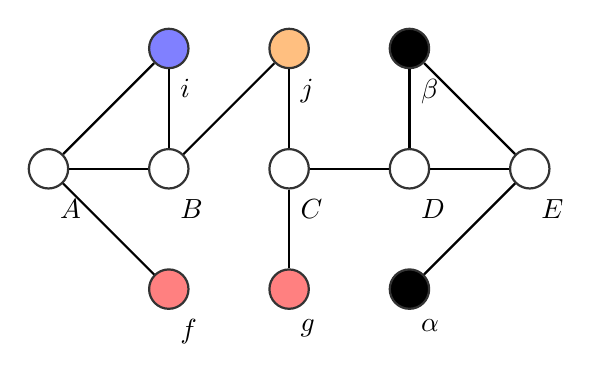
\begin{tikzpicture}
	\tikzstyle{main}=[circle, minimum size = 5mm, thick, draw =black!80, node distance = 10mm]
	\tikzstyle{connect}=[thick]
	\tikzstyle{box}=[rectangle, draw=black!100]
	\node[main, fill = white!100] (a) [            label=275:$A$] { };
	\node[main]                   (b) [right=of a, label=275:$B$] {};
	\node[main]                   (c) [right=of b, label=275:$C$] {};
	\node[main]                   (d) [right=of c, label=275:$D$] {};
	\node[main]                   (e) [right=of d, label=275:$E$] {};
	
	\node[main, fill = red!50]    (f) [below=of b, label=275:$f$] {};	
	\node[main, fill = red!50]    (g) [below=of c, label=275:$g$] {};	
	\node[main, fill = black!100] (h) [below=of d, label=275:$\alpha$] {};
	
	\node[main, fill = blue!50]   (i) [above=of b, label=275:$i$] {};
	\node[main, fill = orange!50] (j) [above=of c, label=275:$j$] {};
	\node[main, fill = black!100] (k) [above=of d, label=275:$\beta$] {};
	
	\path 
	(a) edge [connect] (b)
	(a) edge [connect] (f)
	(a) edge [connect] (i)
	
	(b) edge [connect] (j)
	(j) edge [connect] (c)
	(b) edge [connect] (i)
	
	(c) edge [connect] (d)
	(c) edge [connect] (g)
	
	(d) edge [connect] (k)
	(d) edge [connect] (e)
	(e) edge [connect] (h)
	
	(e) edge [connect] (k)
	;
	
	\end{tikzpicture}
\end{figure}
}

\frame{
	\frametitle{Average Mutational Network Density}
\begin{quote}
	
	To measure Average Network Density, $D_K$:
	
	\begin{enumerate}
		\item enumerate all white nodes (set $K$)
		\item count the proportion of edges to nodes within the phenotype (edges to other white nodes), for each white node in the graph ($\frac{D_k}{nm}$);
		\item calculate the average across all nodes in set $K$ to reflect the relatedness and clustering of the realized genomes in the phenotype.
	\end{enumerate}
	
	\begin{equation}
	D_{K} = {\frac{1}{k} \sum_{i=1}^{k}}\frac{D_k}{nm} 
	\end{equation}
	
\end{quote}
}

\frame{
	\frametitle{Unrealized Network Robustness}
	\begin{quote}
		
		To measure Unrealized Network Robustness, $U_K$:
		\begin{enumerate}
			\item enumerate all white nodes (set $K$)
			\item count the proportion of edges to potential mutants within the phenotype (edges to black nodes), for each white node in the graph ($\frac{U_k}{nm}$);
			\item calculate the average across all nodes in set $K$ to reflect the level of mutational robustness in the population for a given phenotype.
		\end{enumerate}
		
		\begin{equation}
		U_{K} = {\frac{1}{k} \sum_{i=1}^{k}}\frac{U_k}{nm} 
		\end{equation}
	\end{quote}
}

\frame{
	\frametitle{Network Evolvability}
	\begin{quote}
		To measure Network Evolvability, $E_K$:
		\begin{enumerate}
			\item enumerate all white nodes (node $k$ in set $K$)
			\item from each node $k$, count the colored nodes($C$)
			\item for each $k$, calculate the entropy of the edges to colored nodes, to identify the diversity of phenotypes available from that node: $e_k$.
			\item normalize the entropy against the total number of colored node edges to reflect the probability of a genotype connecting to a variety of other phenotypes ($E_k=\frac{{e_{k}}*C}{nm}$).
			\item calculate the average across all nodes in set K to reflect the level of evolvability in the population for a given phenotype.
		\end{enumerate}
		\begin{equation}
		E_{K} = {\frac{1}{k} \sum_{i=1}^{k}} E_k 
		\end{equation}
		
	\end{quote}
		
	}

\section[Experiments]{Experiments}

\frame{
	\frametitle{Avida}
	\begin{figure}[h!]
		\begin{center}
			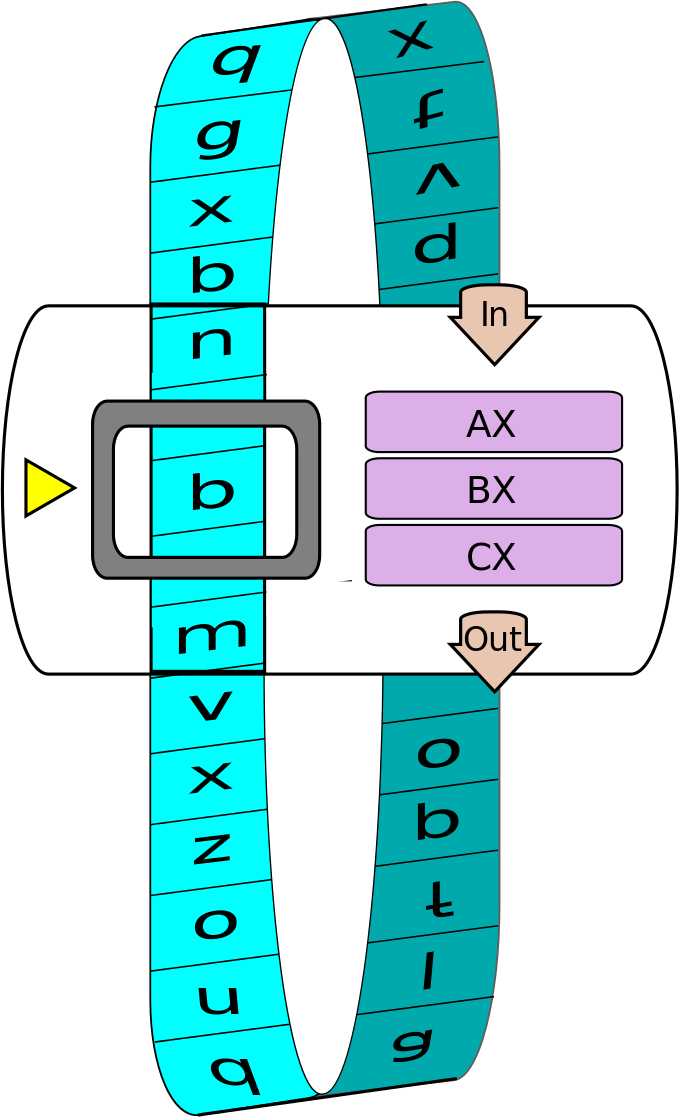
\includegraphics[width=0.27999999999999997\columnwidth]{figures/squishedCPU.png}
			\caption{An example virtual CPU from Avida, with a circular genome (blue), three registers (purple), input and output handlers (tan), and an instruction pointer (yellow) indicating the next instruction to be executed.%
			}\label{fig:cpu}
		\end{center}
	\end{figure}
}

%%%%%%%%%%%%%%%%% SECTION %%%%%%%%%%%%%%%%%%%%%

\subsection[Changing Environments]{Modularity and Evolvability in Changing Environments}

\frame{
	\frametitle{Modularity and Evolvability in Changing Environments}
	\begin{block}{Hypothesis}
	\begin{enumerate}
		\item Changing Environments produce more modular architectural structures than static environments
	\end{enumerate}	
	\end{block}
}

\frame{
	\frametitle{Experimental Design}
			\begin{enumerate}
				\item 150 Replicates, max 3600 individuals
				\item Fixed length organisms
				\item Cyclically changing environment, period of 1000 updates, equal-length phases.
				\item XOR task rewarded continuously
				\item EQU task rewarded/not rewarded according to cycle phase.
				\item Benign treatment - EQU not rewarded during off-cycle
				\item Hostile treatment - EQU punished during off-cycle
				\item Control treatment - No cycle, XOR and EQU always rewarded
			\end{enumerate}	
}

\frame{
	\frametitle{Measurements}
	\begin{enumerate}
		\item Spatial Modularity of Last Common Ancestor (LCA) of Final Population  
		\item Population Phylogenetic Depth
		\item Population Per-Site and Average Genotypic Entropy 
		\item Per-site Task Performance along lineage of LCA.
		\item Proportion of sites related to Tasks
		\item Mutational Landscape
	\end{enumerate}	
}

\frame{
	\frametitle{Results - Evolutionary History}
	\begin{figure}[h!]
		\begin{center}
			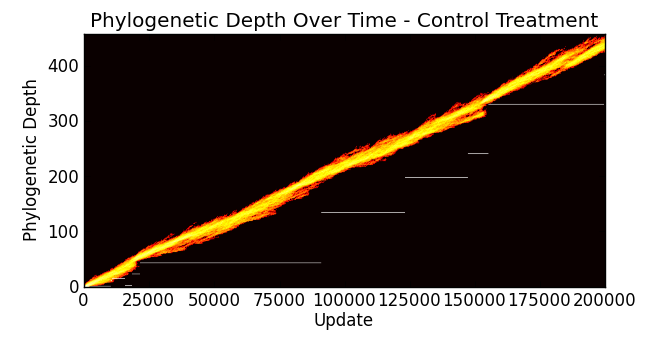
\includegraphics[width=0.45\columnwidth]{figures/flame_graph__control.png}
			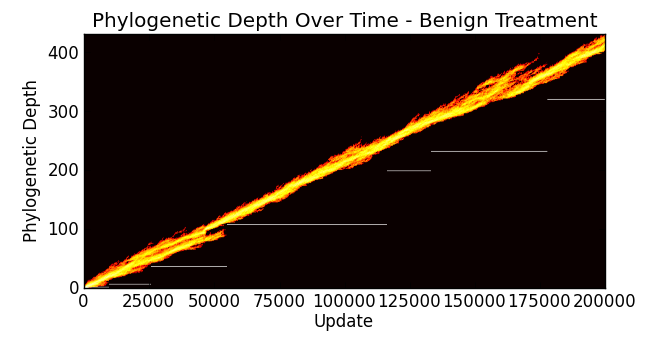
\includegraphics[width=0.45\columnwidth]{figures/flame_graph__benign.png}\\
			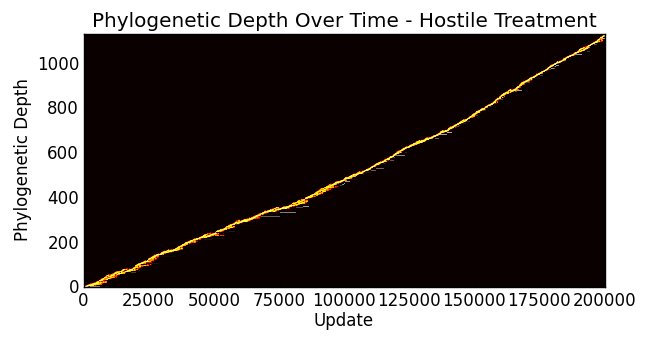
\includegraphics[width=0.9\columnwidth]{figures/flame_graph__hostile.png}\\

		\end{center}
	\end{figure}
}

\frame{
	\frametitle{Per-Site and Average Entropy - Control vs Benign}
	\begin{figure}[h!]
		\begin{center}
			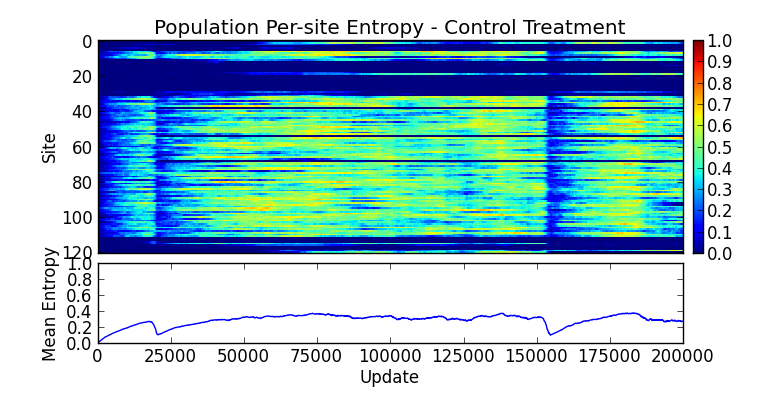
\includegraphics[width=0.7\columnwidth]{figures/by_site_entropy__control.png}\\
			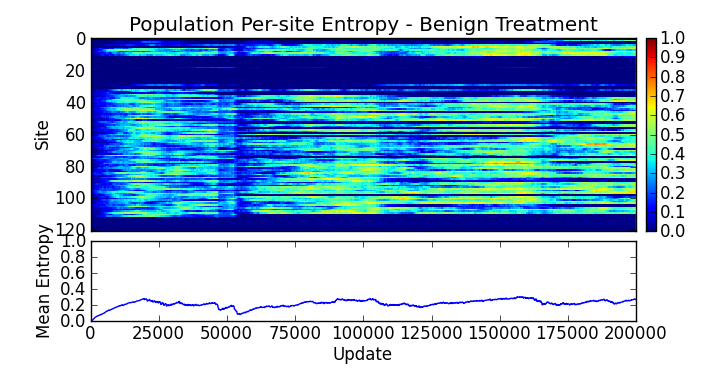
\includegraphics[width=0.7\columnwidth]{figures/by_site_entropy__benign.png}
			
		\end{center}
	\end{figure}
}

\frame{
	\frametitle{Per-Site and Average Entropy - Control vs Hostile}
	\begin{figure}[h!]
		\begin{center}
			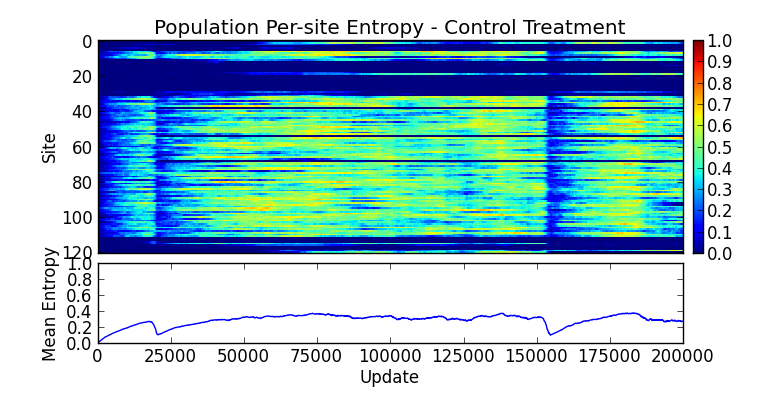
\includegraphics[width=0.7\columnwidth]{figures/by_site_entropy__control.png}\\
			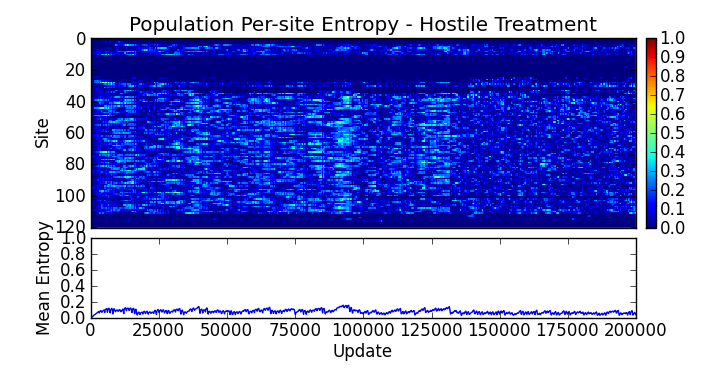
\includegraphics[width=0.7\columnwidth]{figures/by_site_entropy__hostile.png}
			
		\end{center}
	\end{figure}
}

\frame{
	\frametitle{Site Task Execution by Lineage - Control vs Benign}
	\begin{figure}[h!]
		\begin{center}
			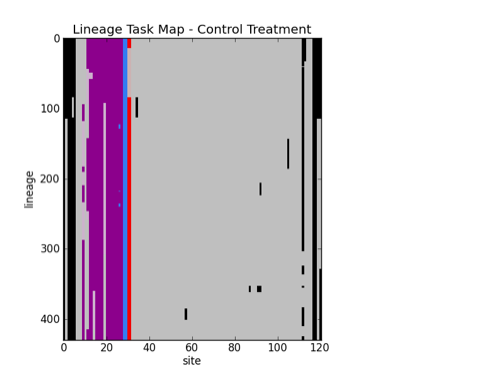
\includegraphics[width=0.45\columnwidth,trim={0.85cm 0 5cm 0},clip]{figures/lineagemap__control.png}
			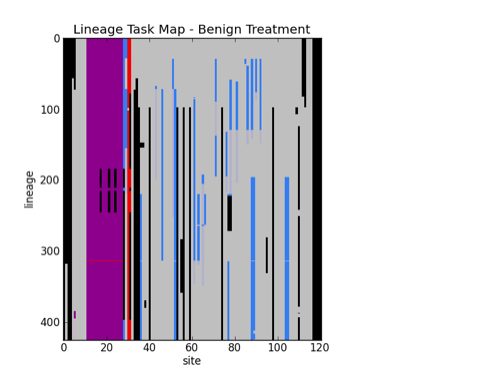
\includegraphics[width=0.45\columnwidth,trim={0.85cm 0 5cm 0},clip]{figures/lineagemap__benign.png}
			
		\end{center}
	\end{figure}
}

\frame{
	\frametitle{Site Task Execution by Lineage - Control vs Hostile}
	\begin{figure}[h!]
		\begin{center}
			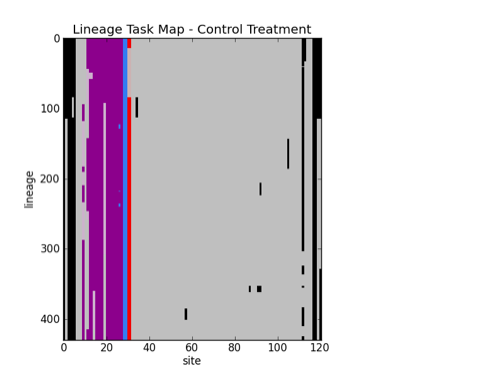
\includegraphics[width=0.45\columnwidth,trim={0.85cm 0 5cm 0},clip]{figures/lineagemap__control.png}
			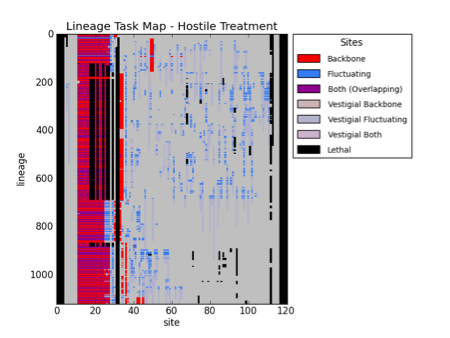
\includegraphics[width=0.6\columnwidth,trim={0.5cm 0 1.3cm 0},clip]{figures/lineagemap__hostile.png}
			%%%% TODO %%%%
			%% fix the caption %%
		\end{center}
	\end{figure}
}
\frame{
	\frametitle{Active and Vestigial Sites}
	\begin{figure}[h!]
		\begin{center}
			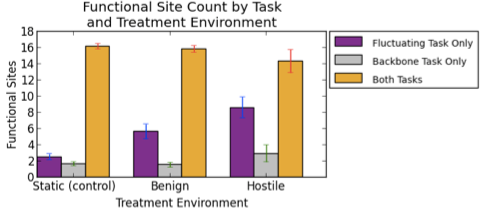
\includegraphics[width=0.7\columnwidth]{figures/site_count__functional.png}
			
			\vspace{0.5cm}
			
			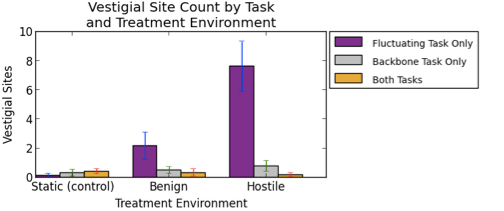
\includegraphics[width=0.7\columnwidth]{figures/site_count__vestigial.png}
			
		\end{center}
	\end{figure}
}
\frame{
	\frametitle{Nearby Mutational Landscape - 1step Mutations - Lost EQU}
	\begin{figure}[h!]
		\begin{center}
			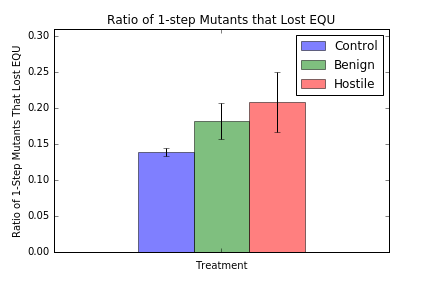
\includegraphics[width=0.7\columnwidth]{figures/one_step_lost_EQU.png}
		\end{center}
	\end{figure}
}

\frame{
	\frametitle{Nearby Mutational Landscape - 2step Mutations - Regained EQU}
	\begin{figure}[h!]
		\begin{center}
			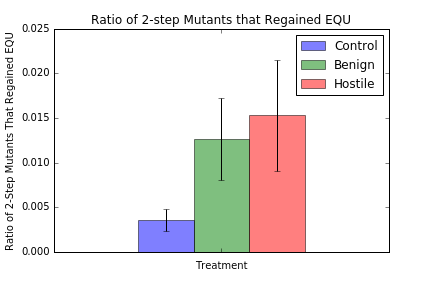
\includegraphics[width=0.7\columnwidth]{figures/two_step_regained_EQU.png}
		\end{center}
	\end{figure}
}

\frame{
	\frametitle{Conclusion}
	\begin{enumerate}
		\item Changing Environments can create quasi-modular structures, de-novo.
		\item Mutationally plastic regions combined with preserved overlapping modules.
		\item Changing Environments shift populations toward more evolvable regions of the mutational landscape.
	\end{enumerate}
}






%%%%%%%%%%%%%%%%%%%%%%%%%%%%%%%%%%%%%%%%%%%%%%%%%%%%%%%%%%%%%%%%%%%%%%%%%%%%%%

\subsection[Sexual Selection]{Sexual Selection and Speciation}

\frame{
	\frametitle{Sexual Selection and Speciation}
	\begin{block}{What is Sexual Selection}
		\begin{enumerate}
			\item MORE HERE TODO
		\end{enumerate}	
	\end{block}
}

\frame{
	\frametitle{Sexual Selection and Speciation}
	\begin{block}{Hypothesis}
		\begin{enumerate}
			\item Sexual Selection increases pre-zygotic isolation during allopatry, resulting in reduced geneflow when populations are rejoined.
		\end{enumerate}	
	\end{block}
}

\frame{
	\frametitle{Experimental Design}
	\begin{enumerate}
		\item 300 Replicates, max 3600 individuals each, in 6 treatments
		\item Evolve in sympatry (single environment) for 100k updates.
		\item Split into two separate populations (Allopatry) for 100k updates.
		\item Rejoined for single round of mating.
		\item 5 treatments with varying task sets during Sympatry and Allopatry, plus all-sympatric control.
	\end{enumerate}	
}

\frame{
	\frametitle{Experimental Design - Treatment Task Sets}
	 \usebeamerfont{small}\begin{figure}[h!]
		\begin{center}
			\begin{tabular}{|l|l|l|l|}
				\hline \textbf{Treatment} & \textbf{Sympatry Tasks} & \textbf{Allopatry Tasks 1} & \textbf{Allopatry Tasks 2} \\
				\hline Control & Logic 9 (all) & N/A & N/A \\
				
				\hline A (restricted) & Logic 9 (all) & \parbox[t]{2cm}{NOT, NAND, AND, ORN, OR, NOR, EQU} & \parbox[t]{2cm}{NOT, NAND, AND, ORN, ANDN, XOR, EQU} \\
				
				\hline B (expanded) & Logic 9 (all)  & \parbox[t]{2cm}{Logic 9 + 3AA, 3AB, 3AC, 3AD} & \parbox[t]{2cm}{Logic 9 + 3BA, 3BB, 3BC, 3BD} \\
				
				\hline C (expanded) & \parbox[t]{2cm}{NOT, NAND, AND, ORN} & \parbox[t]{2cm}{NOT, NAND, AND, OR, NOR, NOR, EQU} & \parbox[t]{2cm}{NOT, NAND, AND, ORN, ANDN, XOR, EQU} \\
				
				\hline D (drift) & Logic 9 (all) & Logic 9 (all) & Logic 9 (all) \\
				
				\hline E (expanded) & \parbox[t]{2cm}{Braided NOT, NAND, AND, ORN} & \parbox[t]{2cm}{NOT, NAND, AND, ORN, OR, NOR, EQU} & \parbox[t]{2cm}{NOT, NAND, AND, ORN, ANDN, XOR, EQU} \\ 
				\hline 
			\end{tabular}
		\end{center}
	\end{figure}
}

\frame{
	\frametitle{Measurements}
	\begin{enumerate}
		\item Hybridization Rates  
		\item Fitness and Viability of Forced-Mating Hybrids
	\end{enumerate}	
}

\frame{
	\frametitle{Results - Pre-zygotic Isolation - Hybridization Rates}
	\begin{figure}[h!]
		\begin{center}
			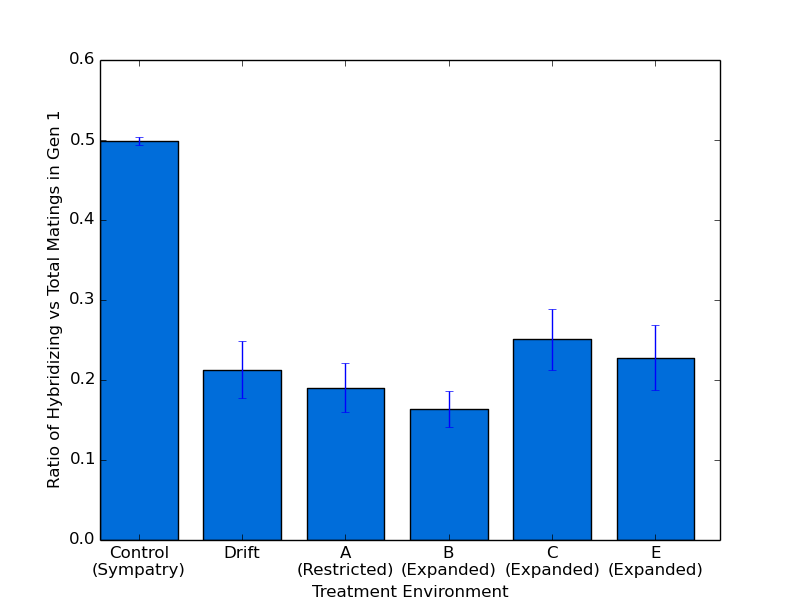
\includegraphics[width=0.7\columnwidth]{figures/118_ratio_sum_matings_gen1__pretty_original.png}
		\end{center}
	\end{figure}
}

\frame{
	\frametitle{Post-Zygotic Isolation - Viability of Offspring from Forced Matings}
	\begin{figure}[h!]
		\begin{center}
			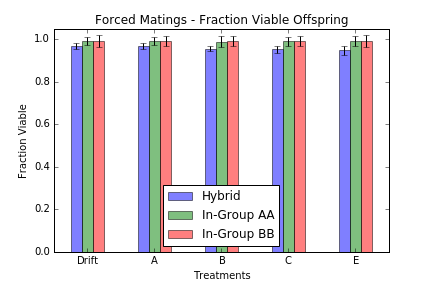
\includegraphics[width=0.7\columnwidth]{figures/recombination_viability.png}
		\end{center}
	\end{figure}
}

\frame{
	\frametitle{Post-Zygotic Isolation - Fitness of Offspring from Forced Matings}
	\begin{figure}[h!]
		\begin{center}
			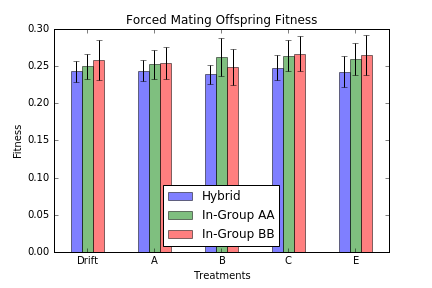
\includegraphics[width=0.7\columnwidth]{figures/recombination_fitness.png}
		\end{center}
	\end{figure}
}

\frame{
	\frametitle{Conclusion}
	\begin{enumerate}
		\item At short time-scales, Sexual Selection increases Pre-zygotic Isolation.
		\item Treatment environment was insufficient to create difference in effect.
	\end{enumerate}
}

%%%%%%%%%%%%%%%%%%%%%%%%%%%%%%%%%%%%%%%%%%%%%%%%%%%%%%%%%%%%%%%%%%%%%%%%%%%%%%

\section[Proposals]{Proposals}

\subsection[HGT]{Proposal: Horizontal Gene Transfer and Modularity}

\frame{
	\frametitle{What is Horizontal Gene Transfer}
	%% TODO %%
}

\frame{
	\frametitle{Hypotheses}
	\begin{enumerate}
		\item Organisms will uptake gene fragments if there is a reward bonus, despite risk of mutation.
		\item Organisms will uptake fragments in environments where evolvability is benificial, even without an energy bonus.
		\item Obligate HGTers will have more modular genomes.
		\item Obligate HGTers will have higher overall fitnesses, and better measures of evolvability.
	\end{enumerate}
}
\frame{
	\frametitle{HGT in Avida}
	\begin{figure}[h!]
		\begin{center}
			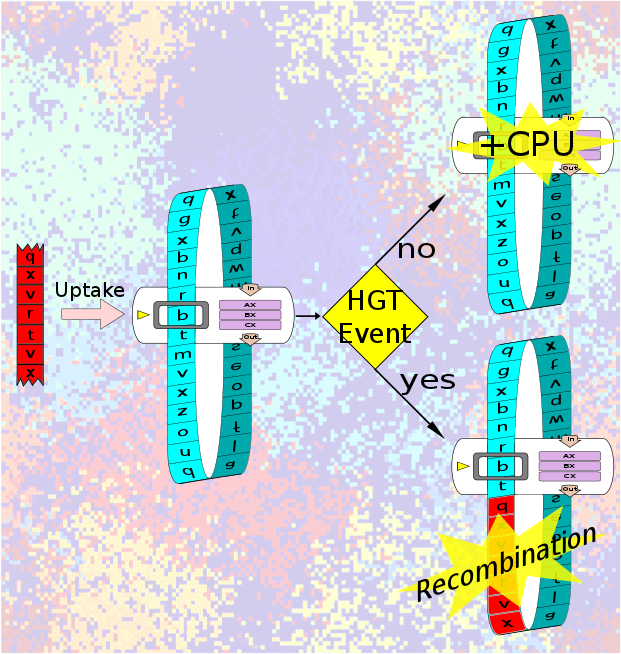
\includegraphics[width=0.7\columnwidth]{figures/Figure.png}
			\caption{The HGT process. Organisms can execute instructions that trigger uptake from the environment. When uptake occurs, there is an experimenter-defined chance that either it will yield a boost to speed of execution or, alternatively, that the fragment will be integrated into the genome.
			}\label{fig:hgtprocess}
		\end{center}
	\end{figure}
}

\frame{
	\frametitle{Proposed Experiments}
	\begin{enumerate}
		\item 50 replicates per treatment, 3600 individuals
		\item Control: No HGT
		\item Treatment 1a: Static environment, Uptake bonus
		\item Treatment 1b: Static environment, No uptake bonus
		\item Treatment 2a: Changing environment, Uptake bonus
		\item Treatment 2a: Changing environment, No uptake bonus
		\item Treatment 3: Obligate HGT
	\end{enumerate}
}
\frame{
	\frametitle{Measurements}
	\begin{enumerate}
		\item HGT Uptake Rates
		\item Spatial and Functional Modularity
		\item Fitness
		\item Evolvability 
	\end{enumerate}
}

%%%%%%%%%%%%%%%%%%%%%%%%%%%%%%%%%%%%%%%%%%%%%%%%%%%%%%%%%%%%%%%%%%%%%%%%%%%%%%
\subsection[Mutational Landscape]{Relating Robustness, Modularity and Evolvability with Mutational Neighborhood Analysis}

\frame{
	\frametitle{Proposal: Relating Robustness, Modularity and Evolvability with Mutational Neighborhood Analysis}
	TBD
}

\frame{
	\frametitle{Research Goals}
	\begin{enumerate}
		\item Explore relationship between mutational landscape and measures of evolvability, modularity, and robustness.
		\item Identify motifs of landscape shape that improve evolvability.
		\item Determine whether mutational landscape network metrics are useful predictors of robustness, evolvability, and modularity.
	\end{enumerate}
}

\frame{
	\frametitle{Proposed Experiments}
	\begin{enumerate}
		\item 50 replicates per treatment, 3600 individuals
		\item Control: Hill-climbing environment, to reduce population diversity effects
		\item Control: Randomly generated neutral networks
		\item Modularity Treatments: Asexual vs Sexual populations
		\item Robustness Treatments 1: High Mutation Rate vs Normal Mutation rates
		\item Robustness Treatments 2: Static Environments vs Changing Environments
	\end{enumerate}
}
\frame{
	\frametitle{Measurements}
	\begin{enumerate}
		\item Neutral Network Density
		\item Network Evolvability, 
		\item Unrealized Network Robustness. 
		\item Spatial and Functional Modularity
		\item Genomic and Phenotypic Robustness
		\item Genomic Diffusion Rate
	\end{enumerate}
}




%%%%%%%%%%%%%%%%%%%%%%%%%%%%%%%%%%%%%%%%%%%%%%%%%%%%%%%%%%%%%%%%%%%%%%
\section[Summary]{Summary}
\frame{
   \frametitle{Summary}
   \begin{enumerate}
  	   \item Evolvability is a complex, overlapping set of concepts.
	   \item Modularity and Robustness may either contribute to or diminish Evolvability depending on their context and scope.
	   \item Network measures for mutational landscapes may provide insights into how to produce more evolvable populations. 
   \end{enumerate}

}


%\section[]{Follow up}
%\frame{
%	\frametitle{There are some possible followup experiments.}
%	\begin{itemize}
%		\item todo
%		\pause
%		\item Remove synonymous mutations.
%		\pause
%		\item Look at more environments.
%		\pause
%		\item Add more degrees of freedom for biases to evolve.
%		\pause
%		\item Look at how mutation bias (doesn't?) change adaptation.
%	\end{itemize}
%}	

\frame{
	\frametitle{Thank you.}
	\begin{block}{Committee Members}
		\begin{tabular}{p{0.5\textwidth} p{0.5\textwidth}}
			Charles Ofria & Chris Adami\\
			Bill Punch & Fred Dyer
		\end{tabular}
	\end{block}
	
%	\begin{block}{DevoLab Members, Past \& Present}
%		\includegraphics[width=\textwidth]{Images/CroppedDevolab.jpg}
%	\end{block}
}


%\frame{
%	\frametitle{Thank you.}
%	\begin{block}{Family \& Friends}
%	\begin{center}
	
%		\includegraphics[height=0.28\textwidth]{Images/JakeAndMe.png}
%		\includegraphics[height=0.28\textwidth]{Images/Family.png}\\
		
%		\includegraphics[height=0.28\textwidth]{Images/IMG_0051.png}
%		\includegraphics[height=0.28\textwidth]{Images/IMG_0056.png}
%	\end{center}
%\end{block}

%}

\begin{frame}[allowframebreaks]{References}
	\usebeamerfont{tiny}
	\bibliography{Comps}
\end{frame}



%\section[Future Work]{Future Work}
%\frame{
%	\frametitle{Future Work}
%	\begin{itemize}
%		\item Look at local landscaping to see the immediate effects of a mutation bias
%		\item Try competing instruction sets with evolved organisms
%		\item Introduce a different mutation bias in a small set of organisms during an experiment
%		\item Use the Path Finding environment
%	\end{itemize}
%}






%\frame{
%	MOAR STUFF.
%	}

%%%%%%%%%%%%%%%%%%%%%%%%%%%%%%%%%%%%%%%%%%%%%%%%%%%%%%%%%%%%%%
	% D R A G O N S    B E    H E R E
%%%%%%%%%%%%%%%%%%%%%%%%%%%%%%%%%%%%%%%%%%%%%%%%%%%%%%%%%%%%%%


\frame{
	Back-end supplemental materials TBD.
}

\end{document}
